%%% main.tex — Deploying ICE-UTxO: Bridge Architecture and Cross-Shard Coordination
\documentclass[11pt,a4paper]{article}
\usepackage[margin=1in]{geometry}
\usepackage{hyperref}
\usepackage{xcolor}

%%% ── Packages ──────────────────────────────────────────────────────────────
\usepackage{amsmath}
\usepackage{amssymb}
\usepackage{mathtools}
\usepackage{stmaryrd}
\usepackage{tikz}
\usepackage{listings}
\usepackage{booktabs}
\usepackage{adjustbox}
\usepackage{cleveref}

%%% ── TikZ libraries ───────────────────────────────────────────────────────
\usetikzlibrary{positioning,arrows.meta,shapes,fit,backgrounds,automata,calc,
                 patterns,decorations.pathreplacing}

%%% ── Shared colour palette (Material Design, desaturated for academic use) ──
\definecolor{palBlue}{HTML}{1976D2}
\definecolor{palBlueLt}{HTML}{E3F2FD}
\definecolor{palGreen}{HTML}{388E3C}
\definecolor{palGreenLt}{HTML}{E8F5E9}
\definecolor{palOrange}{HTML}{E65100}
\definecolor{palOrangeLt}{HTML}{FFF3E0}
\definecolor{palPurple}{HTML}{7B1FA2}
\definecolor{palPurpleLt}{HTML}{F3E5F5}
\definecolor{palRed}{HTML}{C62828}
\definecolor{palRedLt}{HTML}{FFEBEE}
\definecolor{palGray}{HTML}{455A64}
\definecolor{palGrayLt}{HTML}{ECEFF1}
\definecolor{palTeal}{HTML}{00796B}
\definecolor{palTealLt}{HTML}{E0F2F1}

%%% ── Shared TikZ styles ─────────────────────────────────────────────────────
\tikzset{
  stdnode/.style={draw, rounded corners, font=\small, minimum height=0.7cm,
                  inner sep=4pt},
  evtnode/.style={stdnode, minimum height=0.7cm, font=\footnotesize},
  fsmstate/.style={draw, rounded corners, minimum width=1.6cm,
                   minimum height=0.7cm, font=\small},
  modnode/.style={draw, rounded corners, minimum width=2.5cm,
                  minimum height=0.7cm, font=\small},
  actornode/.style={draw, rectangle, minimum width=1.4cm,
                    minimum height=0.7cm, font=\small, thick},
  sortbox/.style={draw, minimum width=0.9cm, minimum height=0.7cm,
                  font=\small},
  layernode/.style={draw, rounded corners, minimum width=9cm,
                    minimum height=1.3cm, align=center, font=\small},
  trackgroup/.style={draw, dashed, rounded corners, inner sep=10pt,
                     fill opacity=0.15},
  stdarrow/.style={-{Stealth[length=5pt]}, thick, shorten >=2pt, shorten <=2pt},
  conflictline/.style={dashed, thick, palRed},
  stutterarrow/.style={dotted, thick, -{Stealth[length=4pt]}},
}

%%% ── Theorem environments ────────────────────────────────────────────────
\usepackage{amsthm}
\newtheorem{theorem}{Theorem}[section]
\newtheorem{lemma}[theorem]{Lemma}
\newtheorem{corollary}[theorem]{Corollary}
\newtheorem{proposition}[theorem]{Proposition}
\newtheorem{remark}[theorem]{Remark}
\newtheorem{definition}[theorem]{Definition}

%%% ── Listings setup for Lean 4 ───────────────────────────────────────────
\lstdefinelanguage{Lean4}{
  morekeywords={theorem,lemma,def,structure,inductive,where,let,have,by,
    import,open,namespace,end,if,then,else,match,with,do,return,sorry,
    axiom,instance,class,extends,section,variable,set_option,example},
  sensitive=true,
  morecomment=[l]{--},
  morecomment=[s]{/-}{-/},
  morestring=[b]",
  literate={→}{$\to$}1 {∀}{$\forall$}1 {∃}{$\exists$}1 {¬}{$\neg$}1
           {∈}{$\in$}1 {∧}{$\wedge$}1 {∨}{$\vee$}1 {≤}{$\leq$}1
           {₀}{$_0$}1 {₁}{$_1$}1 {ₙ}{$_n$}1,
}
\lstset{
  language=Lean4,
  basicstyle=\ttfamily\small,
  keywordstyle=\bfseries,
  commentstyle=\itshape\color{gray},
  breaklines=true,
  frame=single,
  xleftmargin=1em,
  numbers=none,
}

%%% ── Convenience macros ──────────────────────────────────────────────────
\newcommand{\NN}{\mathbb{N}}
\newcommand{\Pfin}{\mathcal{P}_{\text{fin}}}
\newcommand{\ie}{i.e.\@\xspace}
\newcommand{\eg}{e.g.\@\xspace}

%%% ── Title and author ────────────────────────────────────────────────────
\title{Deploying ICE-UTxO:\\Bridge Architecture and Cross-Shard Coordination}

\author{Charles Hoskinson\\
  \textit{Input Output Group}\\
  \texttt{Charles.Hoskinson@gmail.com}
}

\date{}

\begin{document}
\maketitle

\begin{abstract}
ICE-UTxO extends the eUTxO ledger model with coroutines, algebraic effects, and proof-carrying transactions, enabling multi-step, multi-party coordination within single atomic transactions. A companion paper~\cite{PaperA} establishes the formal model and proves its safety properties---serializability, invariant preservation, and conservative extension---in Lean~4.

This paper addresses the deployment architecture. We formalize how coordination scripts (MPST global types with event-structure semantics) are compiled to Programmable Transaction Block programs, integrated with Sharded Byzantine Atomic Commit for cross-shard atomicity, and connected to the ledger commit mechanism via bidirectional bridge theorems. The bridge establishes that shard-local verification of projected traces is both necessary and sufficient for global protocol consistency, enabling each shard to validate only its own roles without replaying the full multiparty execution. The concurrent-to-serial refinement theorem shows that the ledger's interleaved execution---with locks, pending transactions, and effect handlers---faithfully implements a serial specification where transactions commit one at a time.

All compilation and bridge results are mechanized in Lean~4 across three modules (\texttt{PTB.lean}, \texttt{SBAC.lean}, \texttt{Script.lean}), with zero admitted lemmas and zero custom axioms. Trust boundary analysis identifies the irreducible assumptions separating the mechanized proofs from a deployed system: ZK verifier soundness, S-BAC Byzantine tolerance, and network fairness.
\end{abstract}

\noindent\textbf{Keywords:} UTxO, sharded consensus, programmable transaction blocks, multiparty session types, S-BAC, formal verification, Lean~4

\medskip

%% ═══════════════════════════════════════════════════════════════════════════
\section{Introduction}\label{sec:intro}

The ICE-UTxO model~\cite{PaperA} extends eUTxO~\cite{Chakravarty2020} with three layers: coroutine state on UTxOs (enabling multi-step execution), coordination scripts derived from multiparty session types (specifying allowed interactions), and IVC proof artifacts (certifying protocol compliance). The companion paper establishes the formal model and proves safety properties universally in Lean~4: strong conflict serializability, invariant preservation across all eight step constructors, and conservative extension over plain eUTxO.

This paper addresses a question the companion paper deliberately leaves open: how does the formal model connect to a deployable system? Three gaps must be bridged.

\paragraph{From specifications to programs.}
Coordination scripts are event structures---partial orders of events with a conflict relation. On-chain validators need a concrete command sequence. The first gap is compilation: translating event structures to Programmable Transaction Block (PTB) programs with explicit dataflow through result registers, and proving that the translation preserves the event structure's semantics.

\paragraph{From single-shard to multi-shard.}
When a transaction's participants span multiple shards, no single shard can validate the full protocol. The second gap is cross-shard coordination: integrating the coordination witness with Sharded Byzantine Atomic Commit (S-BAC) so that each shard checks only its local projection, and proving that these local checks compose into a global guarantee.

\paragraph{From concurrent to serial.}
The ICE-UTxO ledger allows interleaved execution: transactions can be pending, locked, raising effects, and handling them concurrently. The third gap is refinement: showing that this concurrent execution faithfully implements a serial specification where transactions commit atomically one at a time.

\subsection{Contributions}

\begin{enumerate}
  \item \textbf{PTB compilation} (\cref{sec:ptb}). Formal translation from coordination scripts to PTB programs with mechanized well-formedness, valid-trace, and cross-role safety theorems.

  \item \textbf{S-BAC integration} (\cref{sec:sbac}). Composition of S-BAC with session-type witness verification, with mechanized bidirectional theorems relating global and shard-local validity.

  \item \textbf{MPST-to-ledger bridge} (\cref{sec:bridge}). Trace consistency, cross-role reconstruction, bidirectional witness theorems, and concurrent-to-serial refinement, all mechanized in Lean~4.

  \item \textbf{Trust boundary analysis} (\cref{sec:trust}). Structured identification of assumptions separating the mechanized proofs from deployment, with a per-property trust table.

  \item \textbf{Worked examples} (\cref{sec:ptb-example,sec:sbac-example}). End-to-end compilation and shard-local verification for a collateralized loan liquidation scenario.
\end{enumerate}

\subsection{Paper Roadmap}

\Cref{sec:background} reviews the ICE-UTxO model, PTBs, and S-BAC. \Cref{sec:ptb} formalizes PTB compilation. \Cref{sec:sbac} integrates S-BAC with coordination witnesses. \Cref{sec:bridge} establishes the MPST-to-ledger bridge and concurrent-to-serial refinement. \Cref{sec:trust} analyzes trust boundaries. \Cref{sec:related} surveys related work. \Cref{sec:discussion} discusses limitations and future directions. \Cref{sec:conclusion} concludes.

%% ═══════════════════════════════════════════════════════════════════════════
\section{Background}\label{sec:background}

This section recaps the ICE-UTxO model (established in full in~\cite{PaperA}) and reviews the two external foundations this paper builds on: Programmable Transaction Blocks and Sharded Byzantine Atomic Commit.

\subsection{ICE-UTxO Recap}\label{sec:recap}

ICE-UTxO is a conservative extension of eUTxO. The ledger state consists of a set of live UTxOs, a set of consumed UTxOs, a committed transaction history, and concurrency-control fields (locked inputs, pending transactions, effect queues, handler stacks). Transactions progress through an eight-constructor step relation: \texttt{addPending}, \texttt{lockInputs}, \texttt{installH}, \texttt{raiseE}, \texttt{handleE}, \texttt{uninstallH}, \texttt{commit}, and \texttt{abort}. Two concurrency modes are supported: \emph{locking} (pessimistic, acquiring exclusive locks before commit) and \emph{optimistic} (snapshot isolation with read-set validation at commit time). Safety is maintained by a six-component ledger invariant preserved by every step~\cite[Theorem~4.8]{PaperA}.

Coordination is specified via \emph{scripts}: event structures derived from MPST global types. A script consists of a set of roles, a role-kind assignment, a set of events with associated actions, an order relation (capturing causality), and a conflict relation (capturing mutual exclusion). Scripts are \emph{well-formed} when the order relation is acyclic, the conflict relation is symmetric and irreflexive, and all events and roles are consistently assigned.

Each transaction carries a \emph{coordination witness} $W = (S, \mathit{tr})$ pairing a script $S$ with a trace $\mathit{tr}$ attesting to protocol compliance. The commit guard requires both ledger-level validity (\texttt{commitEnabledStrong}) and witness-level validity (\texttt{witnessGlobalOK}).

\subsection{Programmable Transaction Blocks}\label{sec:ptb-bg}

In standard eUTxO (and Bitcoin), a transaction is a single atomic step: consume inputs, produce outputs. There is no way to express ``first read this UTxO, then use the result to compute something, then write to another UTxO'' as sequential steps within one transaction. Each validator runs independently, seeing only its own datum, redeemer, and the transaction context---there is no mechanism for one validator's output to flow as input to another validator within the same transaction.

\emph{Programmable Transaction Blocks} (PTBs), introduced by Sui~\cite{Blackshear2023}, address this gap by allowing a transaction to contain an ordered sequence of commands with explicit dataflow between them. A PTB is a list of commands $[c_0, c_1, \ldots, c_n]$. Each command $c_i$ performs an operation and stores its result in a register $\mathit{Result}(i)$. Subsequent commands may reference $\mathit{Result}(j)$ for any $j < i$ as input, creating explicit dataflow edges. All commands execute sequentially within one atomic transaction: if any command fails, the entire transaction is reverted. There are no loops or conditional branches within a PTB; any conditional logic must be resolved at transaction construction time.

Other blockchain platforms achieve multi-step execution through different mechanisms. Ethereum handles this implicitly via smart contract code: a single external call can trigger a chain of internal calls, but the ``steps'' are EVM opcodes, not user-visible commands. Solana transactions contain multiple instructions targeting different programs, executing sequentially with shared account state. ICE-UTxO adopts the PTB model as a compilation target because it provides an explicit, inspectable, deterministic schedule well-suited for formal verification and proof generation.

In ICE-UTxO, coordination scripts are compiled to PTB-style programs. The event structure's partial order is linearized into a command sequence with explicit dataflow through result registers: if event $e_j$ causally depends on event $e_i$, then command $c_j$ references $\mathit{Result}(i)$. This compilation step is formalized in \cref{sec:ptb}, with correctness theorems ensuring that the PTB faithfully implements the coordination script's semantics.

\subsection{Sharded Byzantine Atomic Commit}\label{sec:sbac-bg}

When a blockchain's state is \emph{sharded}---partitioned across independent validator sets, each responsible for a disjoint subset of UTxOs---a transaction that touches UTxOs on multiple shards cannot be validated by any single shard alone. Without a coordination protocol, partial execution becomes possible: one shard commits while another rejects, leaving the ledger inconsistent.

Chainspace~\cite{AlBassam2018} introduced \emph{Sharded Byzantine Atomic Commit} (S-BAC), adapting classical two-phase commit for the Byzantine fault-tolerant setting. The protocol operates in two phases. In the \emph{prepare} phase, the transaction is sent to all relevant shards; each shard runs BFT consensus among its validators to check local validity and tentatively locks affected inputs. Each shard votes \emph{prepare} or \emph{abort}. In the \emph{accept} phase, if all shards vote prepare, the coordinator broadcasts \emph{commit}; if any shard votes abort, the coordinator broadcasts \emph{abort}.

S-BAC guarantees \emph{safety unconditionally}: no partial commits can occur, even under Byzantine behaviour by up to $f$ validators per shard ($f < n/3$). \emph{Liveness} requires partial synchrony and honest supermajorities.

In ICE-UTxO, S-BAC is augmented with proof-carrying semantics. During the prepare phase, each shard validates its local projection of the coordination script and checks the IVC witness attached to the transaction. The witness provides cryptographic assurance that the cross-shard data is consistent without requiring shards to re-execute computation performed on remote state.

%% ═══════════════════════════════════════════════════════════════════════════
\section{PTB Compilation}\label{sec:ptb}

A coordination script's event structure admits many valid linearizations---any topological sort of the causal DAG respects the partial order. On-chain validators, however, need a single concrete command sequence to replay and verify. PTB compilation selects one such linearization and encodes it as a Programmable Transaction Block: a sequence of commands where each command produces a result stored in a numbered register $\mathit{Result}(i)$, and later commands reference earlier results as inputs.

The key property is determinism. The event structure captures what \emph{could} happen; the PTB captures what \emph{did} happen. This determinism is what makes on-chain validation possible: validators replay the exact command sequence and verify that the result matches the proof. The correctness criterion is that the PTB's induced event structure is well-formed and admits the PTB's command sequence as a valid trace (Theorems~\ref{thm:toscript-wf}--\ref{thm:valid-trace-trace}). All definitions and theorems are mechanized in \texttt{PTB.lean}.

\subsection{Command Model}\label{sec:command-model}

\begin{definition}[Command]\label{def:command}
A command is a triple $c = (\mathit{action}, \mathit{uses}, \mathit{conflicts})$ where $\mathit{action} : \mathit{Action}$, $\mathit{uses} : \Pfin(\NN)$ identifies result registers consumed as inputs, and $\mathit{conflicts} : \Pfin(\NN)$ records explicit conflict edges.
\end{definition}

\begin{definition}[Program]\label{def:program}
A PTB program is a list of commands $P = [c_0, \ldots, c_{n-1}]$. Command $c_i$ stores its output in register $\mathit{Result}(i)$, and may reference $\mathit{Result}(j)$ for $j \in c_i.\mathit{uses}$. Well-formedness requires $j < i$ for every $j \in c_i.\mathit{uses}$.
\end{definition}

\begin{definition}[Config]\label{def:config}
A PTB configuration $(\mathit{roles}, \mathit{roleKind})$ maps identifiers to roles and roles to kinds, connecting the PTB to the coordination layer's role structure. In the Lean mechanization, an extended variant \texttt{AccessConfig} adds $\mathit{utxoRole}$ and $\mathit{ifaceRole}$ mappings used by the witness construction theorems.
\end{definition}

\subsection{Derived Relations}\label{sec:derived-relations}

Given a program $P$, we derive three dependency relations ($\mathit{dataDep}$, $\mathit{utxoDep}$, $\mathit{handlerDep}$) that contribute to the causal order, plus one conflict marker ($\mathit{explicitConflict}$) for choice branches, and combine these into two structural relations: $\mathit{orderRel}$ (causal order) and $\mathit{conflictRel}$ (mutual exclusion). Each action~$a$ exposes accessor functions: $a.\mathit{readUtxos}$, $a.\mathit{writeUtxos}$, $a.\mathit{consumedUtxos}$, $a.\mathit{ifaceUses}$, $a.\mathit{ifaceInstalls}$, $a.\mathit{ifaceUninstalls}$.

\begin{definition}[Dependencies]\label{def:dependencies}
For commands $c_i, c_j$ with $i < j$:
\begin{itemize}
  \item $\mathit{dataDep}(i, j) \iff i \in c_j.\mathit{uses}$ --- result register dependency.
  \item $\mathit{utxoDep}(i, j) \iff c_i.\mathit{writeUtxos} \cap c_j.\mathit{utxoAccesses} \neq \emptyset \;\lor\; c_j.\mathit{writeUtxos} \cap c_i.\mathit{utxoAccesses} \neq \emptyset$ --- read-write or write-write overlap.
  \item $\mathit{handlerDep}(i, j) \iff c_i.\mathit{ifaceInstalls} \cap c_j.\mathit{ifaceUses} \neq \emptyset \;\lor\; c_i.\mathit{ifaceUses} \cap c_j.\mathit{ifaceUninstalls} \neq \emptyset$ --- install-before-use or use-before-uninstall.
\end{itemize}
\end{definition}

\begin{definition}[Order Relation]\label{def:order-rel}
$\mathit{orderRel}(i, j) \iff i < |P| \wedge j < |P| \wedge i < j \wedge (\mathit{dataDep}(i,j) \lor \mathit{utxoDep}(i,j) \lor \mathit{handlerDep}(i,j))$.
\end{definition}

\begin{definition}[Conflict Relation]\label{def:conflict-rel}
$\mathit{conflictRel}(i, j) \iff i < |P| \wedge j < |P| \wedge i \neq j \wedge (c_i.\mathit{consumedUtxos} \cap c_j.\mathit{consumedUtxos} \neq \emptyset \lor c_i.\mathit{ifaceInstalls} \cap c_j.\mathit{ifaceInstalls} \neq \emptyset \lor \mathit{explicitConflict}(i, j))$.
\end{definition}

\begin{remark}[Hereditary Conflict]\label{rem:conflict-properties}
The relation $\mathit{conflictRel}$ is symmetric and irreflexive but does \emph{not} enforce hereditary conflict (downward closure under causality), as required by Winskel's original event structures~\cite{Winskel1986}. ICE-UTxO omits this because: (i)~PTB-derived event structures have finite, acyclic order relations where acyclicity is sufficient for serializability without hereditary closure; (ii)~the serializability proof~\cite[Theorem~5.5]{PaperA} depends on $\mathit{fullConflicts}$ symmetry and $\mathit{CoreState}$ commutativity, not on hereditary propagation; and (iii)~the projection theorems hold for the weaker conflict relation. For PTB-compiled scripts, the omission has no effect: $\mathit{toScript}$ produces conflict edges only between commands at the same causal depth, so hereditary closure would add no new edges. Adding hereditary closure for hand-written scripts is planned~\cite[Section~8]{PaperA}.
\end{remark}

\subsection{Translation to Event Structure}\label{sec:translation}

\begin{definition}[toScript]\label{def:toscript}
Given configuration $\mathit{cfg}$ and program $P$, the induced script is:
\[
\mathit{toScript}(\mathit{cfg}, P) = (\mathit{cfg}.\mathit{roles}, \mathit{cfg}.\mathit{roleKind}, \{0, \ldots, |P|-1\}, \lambda i.\, c_i.\mathit{action}, \mathit{orderRel}, \mathit{conflictRel})
\]
\end{definition}

\begin{remark}[Compilation Direction]\label{rem:compilation-direction}
The translation is from programs to event structures, not the reverse. The PTB program is the author-facing artifact specifying \emph{what to execute}. The event structure extracted by $\mathit{toScript}$ is the verification artifact specifying \emph{what constraints the execution must satisfy}. A reverse direction---compiling an arbitrary event structure into a PTB---would require solving a scheduling problem and is not needed: transaction authors construct PTB programs directly or via a high-level DSL, and the ledger verifies the induced event structure.
\end{remark}

\begin{theorem}[toScript Well-Formedness]\label{thm:toscript-wf}
If $P$ satisfies $\mathit{rolesOK}$ and $\mathit{roleKindOK}$ with respect to $\mathit{cfg}$, then $\mathit{toScript}(\mathit{cfg}, P)$ is well-formed. \emph{(Mechanized: \texttt{Program.toScript\_wellFormed}, PTB.lean.)}
\end{theorem}

\begin{proof}[Proof sketch]
The seven well-formedness predicates decompose as follows. \textbf{WF-Order} and \textbf{WF-Conflict}: both endpoints are in $\{0, \ldots, |P|-1\}$ by the bound guards in the relation definitions. \textbf{WF-Irrefl} and \textbf{WF-Symm} for conflict: irreflexivity follows from $i \neq j$; symmetry from \texttt{conflictRel\_symm}. \textbf{WF-Acyclic}: if $\mathit{orderRel}^+(i, i)$ held, then $i < i$ by transitivity of the $i < j$ constraint---contradiction. \textbf{WF-Roles} and \textbf{WF-RoleKind}: by hypothesis.
\end{proof}

\subsection{Valid Traces and Witness Construction}\label{sec:valid-traces}

\begin{figure}[t]
\centering
\begin{adjustbox}{max width=\linewidth, center}
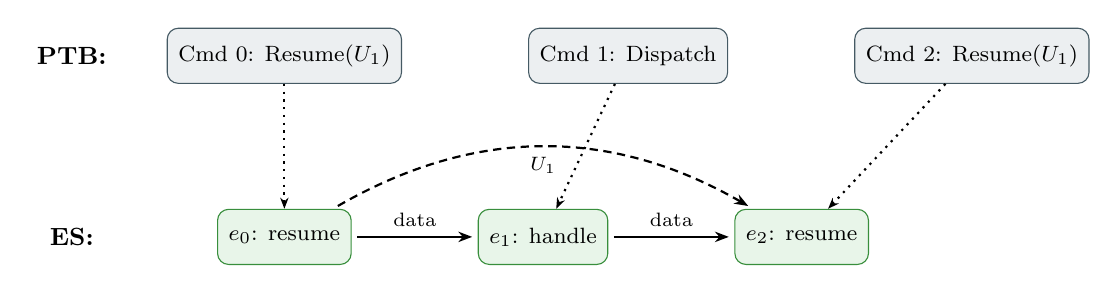
\begin{tikzpicture}[
  node distance=0.8cm and 1.6cm,
  >=Stealth
]
\def\xLabel{-1.2}
\def\xFirst{1.5}
\def\yPTB{1.8}
\def\yES{-0.5}

%% PTB Row
\node[font=\small\bfseries] at (\xLabel, \yPTB) {PTB:};
\node[evtnode, fill=palGrayLt, draw=palGray] (c0) at (\xFirst, \yPTB) {Cmd 0: Resume($U_1$)};
\node[evtnode, fill=palGrayLt, draw=palGray, right=of c0] (c1) {Cmd 1: Dispatch};
\node[evtnode, fill=palGrayLt, draw=palGray, right=of c1] (c2) {Cmd 2: Resume($U_1$)};

%% ES Row
\node[font=\small\bfseries] at (\xLabel, \yES) {ES:};
\node[evtnode, fill=palGreenLt, draw=palGreen] (e0) at (\xFirst, \yES) {$e_0$: resume};
\node[evtnode, fill=palGreenLt, draw=palGreen, right=of e0] (e1) {$e_1$: handle};
\node[evtnode, fill=palGreenLt, draw=palGreen, right=of e1] (e2) {$e_2$: resume};

%% Data Edges
\draw[stdarrow] (e0) -- node[above, font=\scriptsize] {data} (e1);
\draw[stdarrow] (e1) -- node[above, font=\scriptsize] {data} (e2);
\draw[stdarrow, densely dashed, bend left=30] (e0) to node[below, font=\scriptsize] {$U_1$} (e2);

%% Mapping Arrows
\draw[stutterarrow] (c0) -- (e0);
\draw[stutterarrow] (c1) -- (e1);
\draw[stutterarrow] (c2) -- (e2);
\end{tikzpicture}
\end{adjustbox}
\caption{PTB compilation mapping commands to event structures.}
\label{fig:ptb-compilation}
\end{figure}

\begin{theorem}[validTrace\_trace]\label{thm:valid-trace-trace}
If $P$ has no conflicts, then the full program-order trace $[0, \ldots, |P|-1]$ is a valid trace of $\mathit{toScript}(\mathit{cfg}, P)$. \emph{(Mechanized: \texttt{Program.validTrace\_trace}, PTB.lean.)}
\end{theorem}

\begin{theorem}[witnessGlobalOK\_of]\label{thm:witness-global-ok}
If $P$ satisfies $\mathit{rolesOK}$, $\mathit{roleKindOK}$, $\mathit{conflictFree}(\mathit{keep})$, and $\mathit{downClosed}(\mathit{keep})$, then $\mathit{toWitness}(\mathit{cfg}, P, \mathit{keep})$ is globally OK. \emph{(Mechanized: \texttt{Program.witnessGlobalOK\_of}, PTB.lean.)}
\end{theorem}

\begin{theorem}[validTrace\_traceOf]\label{thm:valid-trace-traceof}
Given a predicate $\mathit{keep} : \NN \to \mathit{Bool}$ such that $P$ is conflict-free on $\mathit{keep}$ and $\mathit{keep}$ is down-closed with respect to $\mathit{orderRel}$, the filtered trace $P.\mathit{traceOf}(\mathit{keep})$ is a valid trace of $\mathit{toScript}(\mathit{cfg}, P)$. \emph{(Mechanized: \texttt{Program.validTrace\_traceOf}, PTB.lean.)}
\end{theorem}

\begin{theorem}[crossRoleSafe\_of\_access]\label{thm:cross-role-safe}
If every command's access roles are contained in its participant set ($\mathit{accessRolesOK}$) and explicit conflicts are shared ($\mathit{explicitConflictShared}$), then conflicting commands always share at least one role. \emph{(Mechanized: \texttt{Program.crossRoleSafe\_of\_access}, PTB.lean.)}
\end{theorem}

\paragraph{Choice and the \texttt{keep} predicate.} The predicate $\mathit{keep} : \NN \to \mathit{Bool}$ selects which commands in a PTB are executed in a given run, modeling branching and conditional logic. For a linear protocol (no choices), $\mathit{keep} = \lambda i.\, \mathit{true}$. For a protocol with an exclusive choice between commands $i$ and $j$ (expressed via $\mathit{conflictRel}(i, j)$), exactly one of $\mathit{keep}(i)$ or $\mathit{keep}(j)$ is true. The two well-formedness conditions---$\mathit{keep}$ is conflict-free and down-closed---ensure that the selected subset forms a valid configuration of the induced event structure. The transaction author constructs $\mathit{keep}$ during execution and includes it in the coordination witness. The IVC proof then certifies that the selected commands were executed correctly, binding $\mathit{keep}$ into the $\mathit{commitHash}$.

\subsection{Worked Example: Collateralized Loan}\label{sec:ptb-example}

Consider a collateralized loan liquidation compiled to a 3-command PTB:

\begin{table}[h]
\centering\small
\begin{tabular}{cllcc}
\toprule
$i$ & \textbf{Command} & \textbf{Action} & \textbf{uses} & \textbf{conflicts} \\
\midrule
0 & Resume borrower coroutine & $\texttt{resume}(r_b, r_o, \mathit{oracle}, \mathit{getPrice})$ & $\emptyset$ & $\emptyset$ \\
1 & Dispatch to price handler & $\texttt{raise}(r_o, r_h, \mathit{oracle}, \mathit{dispatch})$ & $\{0\}$ & $\emptyset$ \\
2 & Resume with price result & $\texttt{resume}(r_h, r_b, \mathit{oracle}, \mathit{result})$ & $\{1\}$ & $\emptyset$ \\
\bottomrule
\end{tabular}
\end{table}

\paragraph{Derived edges.} $\mathit{dataDep}(0,1)$ since $0 \in c_1.\mathit{uses}$; $\mathit{dataDep}(1,2)$ since $1 \in c_2.\mathit{uses}$; $\mathit{handlerDep}(0,2)$ since both access the oracle interface. Thus $\mathit{orderRel} = \{(0,1), (1,2), (0,2)\}$ and $\mathit{conflictRel} = \emptyset$.

\paragraph{Induced script.} $\mathit{toScript}$ produces events $\{0,1,2\}$ with order $0 < 1 < 2$ (plus $0 < 2$) and no conflict. This is a total order, so the unique valid trace is $[0,1,2]$.

\paragraph{Validity.} Since $\mathit{conflictRel} = \emptyset$, \cref{thm:valid-trace-trace} applies directly: the program-order trace $[0,1,2]$ is valid. By \cref{thm:witness-global-ok}, $\mathit{toWitness}(\mathit{cfg}, P, \lambda i.\, \mathit{true})$ is globally OK.

\paragraph{Configuration sequence.} Starting from $C_0 = \emptyset$: event~$0$ (resume borrower) is enabled because it has no predecessors and no conflicts, so $C_1 = \{0\}$. Event~$1$ (dispatch to handler) is enabled in $C_1$ because its sole predecessor~$0$ is present, so $C_2 = \{0, 1\}$. Event~$2$ (resume with result) is enabled in $C_2$ because predecessors~$0$ and~$1$ are both present, so $C_3 = \{0, 1, 2\}$. The configuration $C_3$ is maximal.

\paragraph{What the IVC proof certifies.} The transaction author generates an IVC proof certifying: (i)~the borrower's coroutine correctly computed the loan terms from the price data; (ii)~the price-oracle effect was dispatched to the correct handler and the result propagated; and (iii)~the witness $W = (S, [0,1,2])$ satisfies $\mathit{witnessGlobalOK}$. The $\mathit{commitHash}$ binds this proof to the specific input and output UTxOs.

%% ═══════════════════════════════════════════════════════════════════════════
\section{S-BAC Integration}\label{sec:sbac}

When a transaction's participants span multiple shards, the shards must synchronize to ensure atomicity: either all shards commit, or all abort. S-BAC~\cite{AlBassam2018} addresses this with a two-phase protocol. In the prepare phase, each shard independently checks its local portion of the transaction. In the accept phase, if all shards prepared successfully, the transaction commits; otherwise all abort.

ICE-UTxO improves over Chainspace's original design in one key respect: shards only check their local trace conformance (is my role following the protocol?) and UTxO liveness (are the inputs still unspent?). The heavy computation---verifying that the full interleaving respects the coordination script---is certified by the IVC proof, which shards verify rather than re-execute. This reduces both computation overhead and the amount of private data that must be revealed.

\subsection{Formal Definitions}

\begin{definition}[S-BAC Configuration]\label{def:sbac-config}
An S-BAC configuration is a pair $(\mathit{shardOfUtxo}, \mathit{rolesOfShard})$ mapping UTxOs to shards and shards to their associated roles.
\end{definition}

\begin{definition}[Coordination Witness]\label{def:coord-witness}
A coordination witness is a pair $W = (S, \mathit{tr})$ of a script $S$ and a trace $\mathit{tr}$.
\end{definition}

\begin{definition}[Witness Predicates]\label{def:witness-predicates}
\begin{align*}
\mathit{witnessGlobalOK}(W) &\iff S.\mathit{globalConform}(\mathit{tr}) \\
\mathit{witnessLocalOK}(W) &\iff \forall r \in S.\mathit{roles}.\; S.\mathit{localConform}(r, S.\mathit{traceProj}(r, \mathit{tr})) \\
\mathit{witnessConsistent}(W) &\iff S.\mathit{traceConsistent}(\mathit{tr})
\end{align*}
\end{definition}

\begin{definition}[Coordinated Commit]\label{def:coord-commit}
Commit is enabled if the ledger commit guard passes \emph{and} the witness validates:
\[
\mathit{coordCommitEnabled}(m, L, \mathit{ctx}) \iff \mathit{commitEnabledStrong}(m, L, \mathit{tx}) \wedge \mathit{witnessGlobalOK}(W)
\]
\end{definition}

\begin{definition}[Shard-Local Check]\label{def:shard-local-check}
During S-BAC prepare, shard $s$ checks:
\begin{enumerate}
  \item \textbf{Local trace conformance}: for every role $r$ associated with $s$, $\mathit{localConform}(S, r, \mathit{traceProj}(S, r, \mathit{tr}))$.
  \item \textbf{UTxO liveness}: inputs assigned to shard $s$ are in $L.\mathit{utxos}$.
\end{enumerate}
\end{definition}

\subsection{Bidirectional Theorems}

\begin{theorem}[Global Implies Local]\label{thm:global-implies-local}
$\mathit{witnessGlobalOK}(W) \implies \mathit{witnessLocalOK}(W)$. \emph{(Mechanized: \texttt{witnessLocalOK\_of\_global}, SBAC.lean.)}
\end{theorem}

\begin{theorem}[Consistent Implies Global]\label{thm:consistent-implies-global}
If $S$ is well-formed and $\mathit{witnessConsistent}(W)$, then $\mathit{witnessGlobalOK}(W)$. \emph{(Mechanized: \texttt{witnessGlobalOK\_of\_local\_and\_consistent}, SBAC.lean.)}
\end{theorem}

\begin{theorem}[Local Sufficiency]\label{thm:local-sufficiency}
If $\mathit{coordCommitEnabled}(m, L, \mathit{ctx})$ holds, then $\mathit{coordCommitEnabledLocal}(m, L, \mathit{ctx})$ holds; that is, shard-local checks are sufficient when the global witness is valid. \emph{(Mechanized: \texttt{coordCommitEnabledLocal\_of\_global}, SBAC.lean.)}
\end{theorem}

The safety properties established here specify what constitutes a valid execution and prove that the commit mechanism admits only valid executions. Liveness properties---guaranteeing that well-formed protocols eventually complete under fairness assumptions---are established using TLA-style reasoning with model-checking validation~\cite[Section~7]{PaperA}.

\begin{figure}[t]
\centering
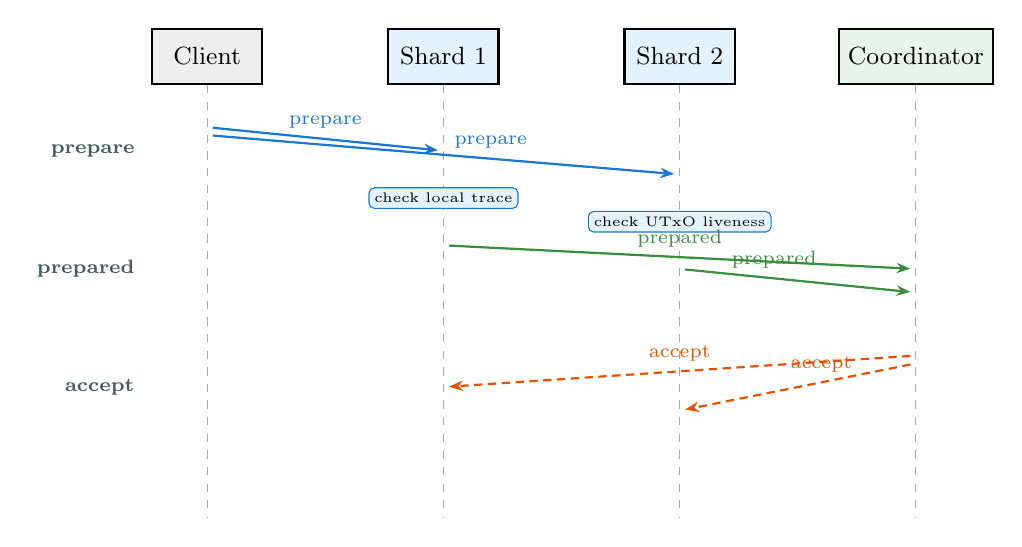
\begin{tikzpicture}[>=Stealth]
\def\xClient{0}    \def\xSOne{3}
\def\xSTwo{6}      \def\xCoord{9}
\def\yPrepare{-1.2}   \def\yPrepared{-2.7}   \def\yAccept{-4.2}

%% Actors
\node[actornode, fill=palGrayLt]  (client) at (\xClient, 0) {Client};
\node[actornode, fill=palBlueLt]  (s1)     at (\xSOne, 0)   {Shard 1};
\node[actornode, fill=palBlueLt]  (s2)     at (\xSTwo, 0)   {Shard 2};
\node[actornode, fill=palGreenLt] (coord)  at (\xCoord, 0)  {Coordinator};

%% Lifelines
\foreach \n in {client, s1, s2, coord} {
  \draw[dashed, palGray!50] (\n.south) -- ++(0, -5.5);
}

%% Phase Labels
\node[font=\scriptsize\bfseries, palGray, anchor=east] at (-0.8, \yPrepare)  {prepare};
\node[font=\scriptsize\bfseries, palGray, anchor=east] at (-0.8, \yPrepared) {prepared};
\node[font=\scriptsize\bfseries, palGray, anchor=east] at (-0.8, \yAccept)   {accept};

%% Messages — Phase 1: prepare
\draw[stdarrow, palBlue] (\xClient, -0.9) -- node[above, font=\scriptsize] {prepare} (\xSOne, \yPrepare);
\draw[stdarrow, palBlue] (\xClient, -1.0) -- node[above, font=\scriptsize, pos=0.6] {prepare} (\xSTwo, -1.5);

% Shard annotations
\node[rounded corners=2pt, fill=palBlueLt, draw=palBlue, font=\tiny, inner sep=2pt]
  at (\xSOne, -1.8) {check local trace};
\node[rounded corners=2pt, fill=palBlueLt, draw=palBlue, font=\tiny, inner sep=2pt]
  at (\xSTwo, -2.1) {check UTxO liveness};

%% Messages — Phase 2: prepared
\draw[stdarrow, palGreen] (\xSOne, -2.4) -- node[above, font=\scriptsize] {prepared} (\xCoord, \yPrepared);
\draw[stdarrow, palGreen] (\xSTwo, \yPrepared) -- node[above, font=\scriptsize, pos=0.4] {prepared} (\xCoord, -3.0);

%% Messages — Phase 3: accept
\draw[stdarrow, densely dashed, palOrange] (\xCoord, -3.8) -- node[above, font=\scriptsize] {accept} (\xSOne, \yAccept);
\draw[stdarrow, densely dashed, palOrange] (\xCoord, -3.9) -- node[above, font=\scriptsize, pos=0.4] {accept} (\xSTwo, -4.5);
\end{tikzpicture}
\caption{S-BAC prepare flow for ICE-UTxO. Three temporal phases flow top-to-bottom.}
\label{fig:sbac}
\end{figure}

\subsection{Worked Example: Cross-Shard Verification}\label{sec:sbac-example}

Continuing the collateralized loan from \cref{sec:ptb-example}, suppose the borrower resides on shard~1 and the oracle on shard~2. Under S-BAC:

\begin{itemize}
  \item \textbf{Shard~1} checks: (i)~$\mathit{witnessLocalOK}$ for the borrower role $r_b$---that the projected trace $[0, 2]$ locally conforms to $\mathit{Proj}(S, r_b)$; and (ii)~that the borrower's input UTxOs are live.
  \item \textbf{Shard~2} checks: $\mathit{witnessLocalOK}$ for oracle role $r_o$ with projected trace $[0, 1]$, and oracle UTxO liveness.
\end{itemize}

By \cref{thm:global-implies-local}, these local checks are implied by global witness validity. By \cref{thm:consistent-implies-global}, their conjunction (plus trace consistency) recovers the global guarantee. Neither shard needs to see the other's UTxO set or re-execute the other's coroutine steps.

%% ═══════════════════════════════════════════════════════════════════════════
\section{MPST-to-Ledger Bridge}\label{sec:bridge}

The preceding sections developed the compilation pipeline (coordination scripts to PTB programs) and the cross-shard integration (S-BAC with proof-carrying witnesses). This section connects the MPST coordination layer to the ledger commit mechanism. The bridge has three parts: trace consistency (\cref{sec:trace-consistency}), coordination witnesses and commit (\cref{sec:coordination-witness}), and concurrent-to-serial refinement (\cref{sec:refinement}).

Without this connection, the MPST types would guarantee protocol structure but say nothing about ledger state, and the ledger invariants would guarantee asset safety but say nothing about whether the protocol was followed.

\subsection{Trace Consistency and Cross-Role Reconstruction}\label{sec:trace-consistency}

Can shard-local verification (checking each role's local trace) reconstruct the global trace consistency needed for commit?

\begin{definition}[Before]\label{def:before}
$\mathit{Before}(\mathit{tr}, a, b) \iff \exists \ell_1, \ell_2.\; \mathit{tr} = \ell_1 \mathbin{+\!\!+} [a] \mathbin{+\!\!+} \ell_2 \wedge b \in \ell_2$.
\end{definition}

\begin{definition}[Trace Consistency]\label{def:trace-consistency}
A trace $\mathit{tr}$ is \emph{consistent} with script $S$, written $S.\mathit{traceConsistent}(\mathit{tr})$, if:
\begin{enumerate}
  \item $\mathit{tr}$ is duplicate-free ($\mathit{tr.Nodup}$)
  \item All events in $\mathit{tr}$ are in $S.\mathit{events}$
  \item No event in $\mathit{tr}$ conflicts with any other event in $\mathit{tr}$
  \item For every order edge $e' < e$ with $e \in \mathit{tr}$, $\mathit{Before}(\mathit{tr}, e', e)$
\end{enumerate}
\end{definition}

These four conditions are the standard requirements for a configuration of an event structure~\cite{Winskel1986}: no duplicates, membership in the event set, conflict-freedom, and causal closure. A trace satisfying these conditions is a linearization of such a configuration.

\begin{definition}[Cross-Role Consistency]\label{def:cross-role}
A trace is \emph{cross-role consistent} if:
\begin{enumerate}
  \item Events with disjoint role sets do not conflict: $\mathit{disjointRoles}(e, f) \implies \neg(e \mathbin{\#} f)$.
  \item Order between disjoint-role events is witnessed: $\mathit{disjointRoles}(e', e) \wedge e' < e \wedge e \in \mathit{tr} \implies \mathit{Before}(\mathit{tr}, e', e)$.
\end{enumerate}
\end{definition}

Local conformance per role ensures that each participant follows its projected protocol. But local conformance says nothing about the relationship between events on disjoint roles. Cross-role consistency fills this gap: condition~(1) requires that events on independent roles do not conflict, and condition~(2) ensures that cross-role causal orderings are respected.

\begin{theorem}[Local + Cross-Role $\Rightarrow$ Global Consistency]\label{thm:local-cross-global}
\begin{align*}
&\mathit{WF}(S) \wedge \mathit{tr.Nodup} \wedge (\forall r \in S.\mathit{roles}.\; \mathit{localConform}(S, r, \mathit{traceProj}(S, r, \mathit{tr}))) \\
&\quad \wedge \mathit{crossRoleConsistent}(S, \mathit{tr}) \implies S.\mathit{traceConsistent}(\mathit{tr})
\end{align*}
\emph{(Mechanized: \texttt{traceConsistent\_of\_local\_and\_cross}, Script.lean.)}
\end{theorem}

\begin{proof}[Proof sketch]
For \emph{conflict-freedom}: given events $a, b$ in $\mathit{tr}$, either they share a role or have disjoint roles. If disjoint, cross-role consistency directly gives $\neg(a \mathbin{\#} b)$. If they share a role $r$, then both appear in $\mathit{traceProj}(S, r, \mathit{tr})$; local conformance implies the local trace is conflict-free, which lifts to the global level.

For \emph{order-respect}: given $e' < e$ with $e \in \mathit{tr}$, case-split on whether $e'$ and $e$ share a role. If disjoint, cross-role consistency provides $\mathit{Before}(\mathit{tr}, e', e)$. If shared via role $r$, local trace validity ensures $e'$ appears before $e$ in the projected trace, which lifts via \texttt{before\_of\_filter}.
\end{proof}

\begin{theorem}[Consistent Implies Valid Trace]\label{thm:consistent-valid}
$S.\mathit{traceConsistent}(\mathit{tr}) \implies S.\mathit{validTrace}(\mathit{tr})$.
\emph{(Mechanized: \texttt{traceConsistent\_implies\_validTrace}.)}
\end{theorem}

\begin{proof}[Proof sketch]
By induction on $\mathit{tr}$, converting consistency evidence into enablement at each step: predecessors present (from order-respect), no conflicts (from pairwise conflict-freedom), event membership (from events check).
\end{proof}

Together, \cref{thm:local-cross-global,thm:consistent-valid} establish a two-step reduction: global trace consistency reduces to per-role local conformance plus cross-role consistency, and any globally consistent trace is a valid execution of the event structure. The practical consequence is that a shard hosting role~$r$ checks only that $r$'s projected trace conforms locally; cross-role conditions are enforced by the coordination witness and the cryptographic proof.

\subsection{Coordination Witness and Commit}\label{sec:coordination-witness}

\begin{theorem}[Bidirectional Witness Theorems]\label{thm:bidirectional}
\begin{enumerate}
  \item \emph{Top-down}: $\mathit{witnessGlobalOK}(W) \implies \mathit{witnessLocalOK}(W)$. A globally valid witness can be verified shard-locally.
  \item \emph{Bottom-up}: $\mathit{WF}(W.\mathit{script}) \wedge \mathit{witnessConsistent}(W) \implies \mathit{witnessGlobalOK}(W)$. If the witness trace is consistent, global conformance follows.
\end{enumerate}
\end{theorem}

\begin{theorem}[Coordinated Commit Implies Local Commit]\label{thm:coord-local}
$\mathit{coordCommitEnabled}(m, L, \mathit{ctx}) \implies \mathit{coordCommitEnabledLocal}(m, L, \mathit{ctx})$.
\emph{(Mechanized: \texttt{coordCommitEnabledLocal\_of\_global}.)}
\end{theorem}

The top-down direction guarantees that a globally valid witness passes every shard's local checks---no honest shard rejects a legitimate transaction. The bottom-up direction guarantees the converse: if every shard independently approves and the trace is consistent, the global protocol was followed. Together they justify decentralized verification: no single authority checks the global protocol end-to-end.

\paragraph{Cross-shard deadlock.} The S-BAC protocol is deadlock-free by construction: each transaction is submitted to all relevant shards simultaneously, and shards respond independently. There is no circular wait because shards do not hold resources across transactions. This depends on three premises: bounded prepare duration (enforced by timeout), unconditional lock release on abort, and the S-BAC coordination protocol being deadlock-free under partial synchrony.

\subsection{Concurrent-to-Serial Refinement}\label{sec:refinement}

We prove that the concurrent ICE-UTxO semantics refines a serial specification where transactions commit atomically one at a time.

\begin{definition}[Serial Step]\label{def:serial-step}
A serial step atomically commits a proof-verified, valid transaction:
\[
\mathit{SerialStep}(m, L, L') \iff \exists \mathit{tx}.\; \mathit{allProofsVerified}(\mathit{tx}) \wedge \mathit{validTx}(L, \mathit{tx}) \wedge \mathit{tx.phase} = \text{Committing} \wedge L' = \mathit{applyCommit}(L, \mathit{tx})
\]
\end{definition}

\begin{definition}[Stuttering]\label{def:stuttering}
A step is \emph{stuttering} if $\mathit{absLedger}(L) = \mathit{absLedger}(L')$. Stuttering steps change only concurrency-control fields without modifying core state.
\end{definition}

\begin{definition}[Abstraction Map]\label{def:abstraction-map}
$\mathit{absLedger}(L) = L[\mathit{locked} := \emptyset, \mathit{pending} := \emptyset, \mathit{effects} := \lambda\_.\, [], \mathit{handlerStacks} := \lambda\_.\, []]$.
\end{definition}

The abstraction map erases exactly the concurrency-control fields: $\mathit{locked}$ (reserved UTxOs during S-BAC prepare), $\mathit{pending}$ (submitted but uncommitted transactions), $\mathit{effects}$ and $\mathit{handlerStacks}$ (algebraic-effect coroutine machinery). None of these exist in the serial specification. The result is that $\mathit{absLedger}(L)$ retains only the UTxO set, consumed set, and committed history.

\begin{theorem}[Concurrent Refines Serial]\label{thm:concurrent-refines-serial}
\[
\mathit{Steps}(m, L_0, L_n) \wedge \mathit{ledgerInvariant}(L_0) \implies \mathit{SerialSteps}(m, \mathit{absLedger}(L_0), \mathit{absLedger}(L_n))
\]
\emph{(Mechanized: \texttt{concurrent\_refines\_serial}, StarstreamPilot.lean.)}
\end{theorem}

\begin{proof}[Proof sketch]
By induction on the \texttt{Steps} derivation. At each step, apply \texttt{step\_preserves\_invariant} to maintain the invariant. Then case-split on the step constructor:
\begin{itemize}
  \item \textbf{Stuttering cases} (7 of 8): \texttt{addPending}, \texttt{lockInputs}, \texttt{abort}, \texttt{installH}, \texttt{uninstallH}, \texttt{raiseE}, \texttt{handleE}. Each has a dedicated lemma showing $\mathit{absLedger}(L) = \mathit{absLedger}(L')$. The serial trace is unchanged.
  \item \textbf{Visible case} (1 of 8): \texttt{commit}. The commit step produces a $\mathit{SerialStep}$ in the abstract trace.
\end{itemize}
\end{proof}

The 7-to-1 split reflects a design principle: seven non-commit constructors manipulate only concurrency-control fields; only \texttt{commit} changes the core state visible to the serial specification. A transaction may raise and handle arbitrarily many effects, install and uninstall multiple handlers, and retry after aborts---an unbounded number of concrete steps---before it eventually commits. The proof requires only that each step either maps to a serial step (commit) or leaves the abstract state unchanged (stuttering).

\begin{figure}[t]
\centering
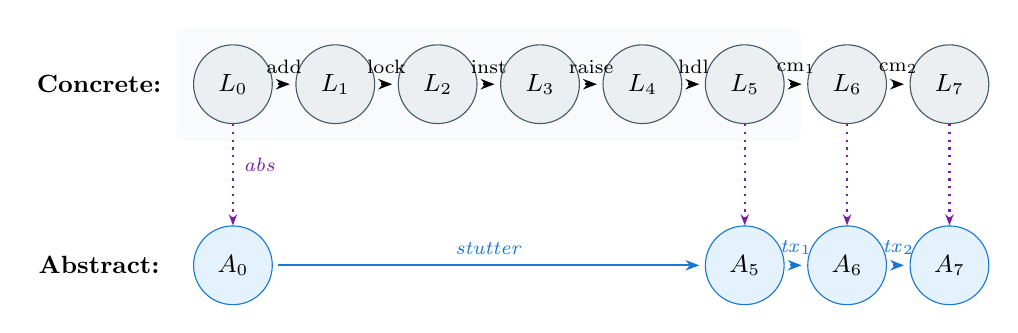
\begin{tikzpicture}[
  cstate/.style={draw, circle, minimum size=1.0cm, font=\small, fill=palGrayLt, draw=palGray},
  astate/.style={draw, circle, minimum size=1.0cm, font=\small, fill=palBlueLt, draw=palBlue},
  >=Stealth,
  node distance=1.2cm
]
\def\yConcrete{1.5}
\def\yAbstract{-0.8}
\def\xSpacing{1.3}

%% Concrete Row
\node[font=\small\bfseries] at (-1.7, \yConcrete) {Concrete:};
\foreach \i/\lbl in {0/L_0, 1/L_1, 2/L_2, 3/L_3, 4/L_4, 5/L_5, 6/L_6, 7/L_7} {
  \node[cstate] (c\i) at (\i*\xSpacing, \yConcrete) {$\lbl$};
}

%% Concrete Edges
\foreach \i/\j/\lbl in {0/1/add,1/2/lock,2/3/inst,3/4/raise,4/5/hdl,5/6/cm$_1$,6/7/cm$_2$} {
  \draw[stdarrow] (c\i) -- node[above, font=\scriptsize] {\lbl} (c\j);
}

%% Stuttering Background
\begin{scope}[on background layer]
  \node[rounded corners, fill=palGrayLt!30, fit=(c0)(c5), inner sep=6pt] {};
\end{scope}

%% Abstract Row
\node[font=\small\bfseries] at (-1.7, \yAbstract) {Abstract:};
\node[astate] (a0) at (c0 |- 0,\yAbstract) {$A_0$};
\node[astate] (a5) at (c5 |- 0,\yAbstract) {$A_5$};
\node[astate] (a6) at (c6 |- 0,\yAbstract) {$A_6$};
\node[astate] (a7) at (c7 |- 0,\yAbstract) {$A_7$};

%% Abstract Edges
\draw[stdarrow, palBlue] (a0) -- node[above, font=\scriptsize] {$\mathit{stutter}$} (a5);
\draw[stdarrow, palBlue] (a5) -- node[above, font=\scriptsize] {$\mathit{tx}_1$} (a6);
\draw[stdarrow, palBlue] (a6) -- node[above, font=\scriptsize] {$\mathit{tx}_2$} (a7);

%% Abstraction Map
\draw[stutterarrow, palPurple] (c0) -- node[right, font=\scriptsize, pos=0.4] {$\mathit{abs}$} (a0);
\draw[stutterarrow, palPurple] (c5) -- (a5);
\draw[stutterarrow, palPurple] (c6) -- (a6);
\draw[stutterarrow, palPurple] (c7) -- (a7);
\end{tikzpicture}
\caption{Refinement diagram: concrete concurrent steps map to abstract serial steps via $\mathit{absLedger}$. Non-commit steps are stuttering.}
\label{fig:refinement}
\end{figure}

The predicate $\mathit{refinementWitness}(m, L, \mathit{tx})$ bundles the conditions under which a concrete commit step corresponds to an abstract serial step: (a)~the witness is globally valid, (b)~all proofs are verified, (c)~the transaction is structurally valid, and (d)~the transaction is in the Committing phase. This is $\mathit{coordCommitEnabled}$ restricted to a single transaction.

\begin{theorem}[Circuit Witness Implies Serial Step]\label{thm:circuit-serial}
$\mathit{refinementWitness}(m, L, \mathit{tx}) \implies \mathit{SerialStep}(m, L, \mathit{applyCommit}(L, \mathit{tx}))$.
\emph{(Mechanized: \texttt{circuit\_witness\_implies\_serial\_step}.)}
\end{theorem}

The results of this section establish a layered correctness argument. Trace consistency and the bidirectional witness theorems ensure that shard-local verification is sound and complete with respect to the global MPST protocol. The refinement theorem then shows that committed transactions form a serial history. Combined with the conflict serializability result from~\cite[Section~5]{PaperA}, this gives a two-level guarantee: the committed history is serializable, and each transaction faithfully implements its declared multiparty protocol.

The bridge relies on assumptions stated in the companion paper: (i)~ZK verifier soundness; (ii)~S-BAC shard honesty ($f < n/3$ Byzantine validators per shard); and (iii)~well-formedness of the global script. The S-BAC protocol itself is not mechanized in Lean; its correctness is assumed from the established literature~\cite{AlBassam2018}. Formally verifying the S-BAC layer---perhaps using Verdi-style verified system transformers~\cite{Wilcox2015}---would close this remaining gap.

%% ═══════════════════════════════════════════════════════════════════════════
\section{Trust Boundaries}\label{sec:trust}

The mechanization makes three trust-boundary assumptions explicit, marked with inline comments in the Lean source code. Each defines the boundary between what the model proves and what it assumes from the external environment.

\paragraph{F3: The verifier oracle.}
The predicate $\mathit{allProofsVerified}(\mathit{tx})$ checks that every \texttt{ProofCommitment} attached to a transaction has reached the \texttt{Verified} phase. The model does not define what a valid proof \emph{is}---it trusts that the external verifier labels correctly. Every safety theorem is conditional on this oracle. If the ZK circuit has a soundness bug, the formal guarantees do not hold.

\paragraph{F5: UTxO immutability justifies read-set validation.}
The predicate $\mathit{readSetValid}$ checks $\mathit{tx.readSet} \subseteq l.\mathit{utxos}$---a pure existence check. In an account-based model this would be insufficient for snapshot isolation because balances can change between read and commit. In the UTxO model, each UTxO is immutable from creation to consumption: its value, datum, and validator reference never change. An existence check therefore \emph{is} a snapshot-consistency check.

\paragraph{F9: Asynchronous handler registration.}
The function $\mathit{handleEffect}$ returns $\mathit{none}$ when no handler is installed for an interface, preventing the \texttt{handleE} step from firing. Effects remain queued until $\mathit{installH}$ pushes a handler. The event-structure causal order guarantees that $\mathit{installH}$ precedes $\mathit{handleE}$ for the same interface; the liveness argument guarantees eventual handling under fair scheduling.

\paragraph{External assumptions.}
Beyond the code-level boundaries, the mechanization relies on three external assumptions: (i)~IVC/SNARK soundness---no adversary can produce a valid proof for a false statement; (ii)~S-BAC shard honesty---fewer than one-third Byzantine validators per shard; and (iii)~network fairness---weak fairness for commit and abort actions, eventual message delivery for cross-shard coordination. Every safety theorem is conditional on~(i); every liveness claim is conditional on~(ii) and~(iii).

\subsection{Per-Property Trust Table}

\begin{table}[t]
\caption{Trust requirements per property. ``Proved'' means mechanized in Lean with zero sorry; ``Assumed'' means the property relies on the indicated external assumption.}
\label{tab:trust}
\centering\small
\begin{tabular}{p{4.5cm}ccc}
\toprule
\textbf{Property} & \textbf{ZK Sound} & \textbf{S-BAC Honest} & \textbf{Fair Sched.} \\
\midrule
No double spend & Proved & --- & --- \\
Invariant preservation & Proved & --- & --- \\
Conflict serializability & Proved & --- & --- \\
Conservative extension & Proved & --- & --- \\
Commit requires proof & Proved & Assumed & --- \\
Global $\Leftrightarrow$ local witness & Proved & --- & --- \\
Local sufficiency & Proved & Assumed & --- \\
Concurrent-to-serial refinement & Proved & --- & --- \\
Eventual commit & --- & Assumed & Assumed \\
Eventual termination & --- & --- & Assumed \\
Eventual effect handling & --- & --- & Assumed \\
Cross-shard atomicity & --- & Assumed & Assumed \\
\bottomrule
\end{tabular}
\end{table}

\Cref{tab:trust} summarizes which external assumptions each property depends on. The core safety properties (no double spend, invariant preservation, serializability, conservative extension) are proved unconditionally in Lean. Properties involving the commit mechanism additionally assume ZK verifier soundness. Cross-shard properties assume S-BAC Byzantine tolerance. Liveness properties assume fair scheduling and, for cross-shard transactions, S-BAC liveness.

%% ═══════════════════════════════════════════════════════════════════════════
\section{Related Work}\label{sec:related}

\subsection{Sharded Consensus and Cross-Shard Coordination}

Al-Bassam et al.~\cite{AlBassam2018} introduce Chainspace, a sharded smart-contract platform using S-BAC to execute transactions spanning multiple shards. ICE-UTxO adopts S-BAC but adds protocol-level verification: each sub-transaction carries a proof witness derived from the MPST projection, and the atomic-commit decision incorporates witness validation alongside the usual safety checks. This means cross-shard transactions respect not only ledger-level invariants but also application-level protocol structure.

OmniLedger~\cite{KokorisKogias2018} uses a similar two-phase structure with client-driven coordination and lock-unlock semantics. Cosmos IBC provides asynchronous cross-chain messaging with timeout-based rollback, trading strong consistency for availability. Polkadot's relay-chain model achieves cross-shard finality through unified consensus at the relay layer. ICE-UTxO's contribution is orthogonal to the choice of commit protocol: we show how to layer session-type verification on top of any atomic-commit primitive.

\paragraph{Hydra.}
Input Output Global's Hydra~\cite{Hydra2023} provides isomorphic state channels for Cardano, enabling off-chain transaction processing among a fixed set of participants. Hydra heads maintain a local ledger that mirrors the main chain's eUTxO semantics, with the main chain serving as a dispute resolution layer. The key difference from ICE-UTxO is scope: Hydra optimizes throughput for a \emph{fixed participant set} by moving computation off-chain, while ICE-UTxO enables \emph{dynamic multiparty coordination} on-chain via session-typed protocols. The approaches are complementary: Hydra could serve as a fast execution layer for ICE-UTxO transactions among co-located participants, with the main chain providing finality and cross-shard coordination via S-BAC.

\subsection{Proof-Carrying Transactions and IVC}

ZEXE~\cite{Bowe2018} introduced proof-carrying transactions for blockchains, where each transaction carries a zero-knowledge proof certifying that its state transition satisfies application-specific predicates. Aleo~\cite{Aleo2021} deploys this in production using a record-based model. Mina~\cite{Mina2020} uses recursive SNARK composition for a constant-size blockchain.

Nova~\cite{Kothapalli2022} and HyperNova~\cite{Kothapalli2023} are the IVC folding schemes that make incremental proof generation practical, enabling per-step proof folding with dramatically lower proving costs. This is directly relevant to ICE-UTxO: each coroutine yield/resume step can be folded into the running IVC accumulator.

ICE-UTxO's proofs specifically certify multiparty session protocol compliance---that the schedule of operations respected the causal order and conflict relations specified by the coordination script. This is more structured than general-purpose proof-carrying data, enabling shard-local verification and composability.

\paragraph{Lurk.}
Lurk~\cite{Lurk2022} provides a Turing-complete language for recursive zk-SNARKs, enabling general-purpose computation to be certified incrementally. Lurk's approach to content-addressed, verifiable computation is relevant to ICE-UTxO's proof layer: Lurk could serve as an implementation substrate for the IVC proof generation that ICE-UTxO requires, providing a production-ready proving backend for coordination script compliance.

\subsection{Mechanized Proofs of Distributed Systems}

IronFleet~\cite{Hawblitzel2015} demonstrates end-to-end verification of distributed systems in Dafny. ICE-UTxO adopts a similar two-layer decomposition---event-structure semantics as the protocol layer, UTxO operational semantics as the implementation layer---but derives the protocol layer from MPST rather than hand-written state machines.

Verdi~\cite{Wilcox2015} provides a Coq framework using verified system transformers. ICE-UTxO's S-BAC layer is analogous to a Verdi transformer that lifts ideal-model guarantees to a Byzantine setting. Formally verifying S-BAC using Verdi-style transformers is a natural direction for future work.

Aneris~\cite{KroghJespersen2020} builds on Iris separation logic for distributed systems reasoning. ICE-UTxO's concurrency is mediated entirely by the ledger (UTxO consumption is the sole synchronisation primitive), so the fine-grained local-concurrency reasoning Iris provides is not required, but Aneris's protocol logic could complement ICE-UTxO for modeling network-level interaction.

\subsection{UTxO Models and Blockchain Verification}

Chakravarty et al.~\cite{Chakravarty2020} introduce eUTxO; Melkonian et al.~\cite{Melkonian2019} provide a mechanized reference semantics in Agda. ICE-UTxO extends both with session-type indexing and proof-carrying transactions, and additionally proves the correspondence between event-structure and operational semantics.

Sui's Move language~\cite{Blackshear2019} adopts an object-centric model with programmable transaction blocks~\cite{Blackshear2023} for atomic multi-operation composition. ICE-UTxO differs in employing MPST for protocol-level safety, ensuring not only that individual resources are used correctly but that the overall multi-party interaction adheres to a choreographic specification.

P\^{i}rlea and Sergey~\cite{PirleaSergey2023} mechanize blockchain consensus properties in Coq; their work is complementary to our Lean~4 mechanization and demonstrates the growing maturity of machine-checked proofs for distributed ledger systems.

Park et al.~\cite{Park2018} provide formal verification tools for Ethereum VM bytecode, targeting a different layer of the verification stack (execution correctness vs.\ protocol compliance) but sharing the goal of machine-checked guarantees for blockchain systems.

%% ═══════════════════════════════════════════════════════════════════════════
\section{Discussion and Future Work}\label{sec:discussion}

\paragraph{Verifying S-BAC.}
The S-BAC protocol is specified at the predicate level (\texttt{SBAC.lean}) but not verified as a distributed protocol. Mechanizing message passing, quorum voting, and Byzantine fault tolerance---perhaps using Verdi's verified system transformers~\cite{Wilcox2015}---would close the gap between the mechanized proofs and a deployed system.

\paragraph{Performance.}
Per-transaction SNARK proof generation remains computationally expensive. Even with Nova's folding~\cite{Kothapalli2022}, generating the final proof for a complex multi-step transaction may require hundreds of milliseconds to seconds on commodity hardware. Verification is fast (typically under 10ms), so on-chain costs are modest, but the proving burden falls on transaction authors. Hardware acceleration, batched proof generation, and proof delegation to sophisticated participants are available mitigations. Empirical benchmarking on representative coordination scenarios is left to future work.

\paragraph{Resource accounting.}
Gas, compute budgets, and memory limits are outside the current scope. Adding a fuel argument to the step relation would formalize resource exhaustion as an abort condition without affecting the existing safety theorems.

\paragraph{DSL and tooling.}
Production adoption requires a high-level domain-specific language hiding the formal machinery---a Scribble-like~\cite{Yoshida2014} protocol description language that generates the MPST global type, PTB program, and IVC circuit constraints automatically. IDE integration, application-domain error messages, and automated testing support are prerequisites for developer adoption.

\paragraph{Incentive compatibility.}
MPST guarantees deadlock freedom but not that all parties cooperate. A malicious party can refuse to execute, causing timeout and abort. The abort constructor ensures safety (no partial state changes are committed), but repeated aborts impose opportunity costs on honest participants. Stake bonds, reputation systems, or economic penalties could mitigate griefing. Formalizing incentive compatibility is a substantial research direction.

\paragraph{Integration with existing chains.}
Connecting ICE-UTxO to Cardano's Plutus or Sui's PTB runtime requires bridging the idealized model and concrete constraints: gas limits, transaction size bounds, serialization formats, and network protocols. Coroutine frames would reside in UTxO datum fields subject to size limits. These constraints bound practical complexity but do not affect the formal model's safety guarantees.

%% ═══════════════════════════════════════════════════════════════════════════
\section{Conclusion}\label{sec:conclusion}

This paper establishes the deployment architecture connecting ICE-UTxO's formal model to a sharded blockchain system. Three results form the backbone.

First, PTB compilation translates coordination scripts (MPST global types with event-structure semantics) to concrete Programmable Transaction Block programs with explicit dataflow, and mechanized theorems prove that the translation preserves well-formedness, valid traces, and cross-role safety.

Second, S-BAC integration composes Sharded Byzantine Atomic Commit with session-type witness verification, with bidirectional theorems showing that global witness validity and shard-local validity are equivalent under well-formedness and trace consistency. This decomposition is what makes shard-local verification scalable: each shard checks only its own roles, and the coordination witness ensures local checks compose into a global guarantee.

Third, the MPST-to-ledger bridge connects the coordination layer to the ledger commit mechanism via trace consistency, cross-role reconstruction, and concurrent-to-serial refinement. The refinement theorem shows that the concurrent ledger---with locks, pending transactions, and effect handlers---faithfully implements a serial specification where transactions commit one at a time. Combined with the conflict serializability result from the companion paper~\cite{PaperA}, this gives a two-level guarantee: committed histories are serializable, and each transaction faithfully implements its declared protocol.

Trust boundary analysis identifies the irreducible assumptions: ZK verifier soundness, S-BAC Byzantine tolerance, and network fairness. Core safety properties are proved unconditionally; cross-shard and liveness properties are conditional on these assumptions. Mechanizing the S-BAC layer and providing empirical performance benchmarks are the most important remaining steps toward deployment.

%% ═══════════════════════════════════════════════════════════════════════════
\bibliographystyle{plain}
\bibliography{references}

\end{document}
